\documentclass[journal,12pt,twocolumn]{IEEEtran}

\usepackage{setspace}
\usepackage{gensymb}
\singlespacing
\usepackage[cmex10]{amsmath}

\usepackage{amsthm}

\usepackage{mathrsfs}
\usepackage{txfonts}
\usepackage{stfloats}
\usepackage{bm}
\usepackage{cite}
\usepackage{cases}
\usepackage{subfig}

\usepackage{longtable}
\usepackage{multirow}

\usepackage{enumitem}
\usepackage{mathtools}
\usepackage{steinmetz}
\usepackage{tikz}
\usepackage{circuitikz}
\usepackage{verbatim}
\usepackage{tfrupee}
\usepackage[breaklinks=true]{hyperref}
\usepackage{graphicx}
\usepackage{tkz-euclide}

\usetikzlibrary{calc,math}
\usepackage{listings}
    \usepackage{color}                                            %%
    \usepackage{array}                                            %%
    \usepackage{longtable}                                        %%
    \usepackage{calc}                                             %%
    \usepackage{multirow}                                         %%
    \usepackage{hhline}                                           %%
    \usepackage{ifthen}                                           %%
    \usepackage{lscape}     
\usepackage{multicol}
\usepackage{chngcntr}

\DeclareMathOperator*{\Res}{Res}
\renewcommand\thesection{\arabic{section}}
\renewcommand\thesubsection{\thesection.\arabic{subsection}}
\renewcommand\thesubsubsection{\thesubsection.\arabic{subsubsection}}

\renewcommand\thesectiondis{\arabic{section}}
\renewcommand\thesubsectiondis{\thesectiondis.\arabic{subsection}}
\renewcommand\thesubsubsectiondis{\thesubsectiondis.\arabic{subsubsection}}


\hyphenation{op-tical net-works semi-conduc-tor}
\def\inputGnumericTable{}                                 %%

\newtheorem{theorem}{Theorem}[section]
\newtheorem{problem}{Problem}
\newtheorem{proposition}{Proposition}[section]
\newtheorem{lemma}{Lemma}[section]
\newtheorem{corollary}[theorem]{Corollary}
\newtheorem{example}{Example}[section]
\newtheorem{definition}[problem]{Definition}

\newcommand{\BEQA}{\begin{eqnarray}}
\newcommand{\EEQA}{\end{eqnarray}}
\newcommand{\define}{\stackrel{\triangle}{=}}
\bibliographystyle{IEEEtran}
\raggedbottom
\setlength{\parindent}{0pt}
\providecommand{\mbf}{\mathbf}
\providecommand{\pr}[1]{\ensuremath{\Pr\left(#1\right)}}
\providecommand{\qfunc}[1]{\ensuremath{Q\left(#1\right)}}
\providecommand{\sbrak}[1]{\ensuremath{{}\left[#1\right]}}
\providecommand{\lsbrak}[1]{\ensuremath{{}\left[#1\right.}}
\providecommand{\rsbrak}[1]{\ensuremath{{}\left.#1\right]}}
\providecommand{\brak}[1]{\ensuremath{\left(#1\right)}}
\providecommand{\lbrak}[1]{\ensuremath{\left(#1\right.}}
\providecommand{\rbrak}[1]{\ensuremath{\left.#1\right)}}
\providecommand{\cbrak}[1]{\ensuremath{\left\{#1\right\}}}
\providecommand{\lcbrak}[1]{\ensuremath{\left\{#1\right.}}
\providecommand{\rcbrak}[1]{\ensuremath{\left.#1\right\}}}
\theoremstyle{remark}
\newtheorem{rem}{Remark}
\newcommand{\sgn}{\mathop{\mathrm{sgn}}}
% \providecommand{\abs}[1]{\left\vert#1\right\vert}
\providecommand{\res}[1]{\Res\displaylimits_{#1}} 
% \providecommand{\norm}[1]{\left\lVert#1\right\rVert}
%\providecommand{\norm}[1]{\lVert#1\rVert}
\providecommand{\mtx}[1]{\mathbf{#1}}
% \providecommand{\mean}[1]{E\left[ #1 \right]}
\providecommand{\fourier}{\overset{\mathcal{F}}{ \rightleftharpoons}}
%\providecommand{\hilbert}{\overset{\mathcal{H}}{ \rightleftharpoons}}
\providecommand{\system}{\overset{\mathcal{H}}{ \longleftrightarrow}}
	%\newcommand{\solution}[2]{\textbf{Solution:}{#1}}
\newcommand{\solution}{\noindent \textbf{Solution: }}
\newcommand{\cosec}{\,\text{cosec}\,}
\providecommand{\dec}[2]{\ensuremath{\overset{#1}{\underset{#2}{\gtrless}}}}
\newcommand{\myvec}[1]{\ensuremath{\begin{pmatrix}#1\end{pmatrix}}}
\newcommand{\mydet}[1]{\ensuremath{\begin{vmatrix}#1\end{vmatrix}}}
\numberwithin{equation}{subsection}
\makeatletter
\@addtoreset{figure}{problem}
\makeatother
\let\StandardTheFigure\thefigure
\let\vec\mathbf
\renewcommand{\thefigure}{\theproblem}
\def\putbox#1#2#3{\makebox[0in][l]{\makebox[#1][l]{}\raisebox{\baselineskip}[0in][0in]{\raisebox{#2}[0in][0in]{#3}}}}
     \def\rightbox#1{\makebox[0in][r]{#1}}
     \def\centbox#1{\makebox[0in]{#1}}
     \def\topbox#1{\raisebox{-\baselineskip}[0in][0in]{#1}}
     \def\midbox#1{\raisebox{-0.5\baselineskip}[0in][0in]{#1}}

\lstset{
%language=C,
frame=single, 
breaklines=true,
columns=fullflexible
}
\title{Assignment 3}
\author{Varenya Upadhyaya EP20BTECH11026}
\date{}
\begin{document}

\maketitle
Download all python codes from:
\begin{lstlisting}
https://github.com/varenya27/AI1103/blob/main/Assignment3/codes
\end{lstlisting}
and all latex-tikz codes from:
\begin{lstlisting}
https://github.com/varenya27/AI1103/blob/main/Assignment3/main.tex
\end{lstlisting}
\maketitle   
\begin{center}
\section*{\textbf{Problem}}
\end{center}
Let (X,Y) be the coordinates of a point chosen at random inside the disc $x^2 + y^2 \leq r^2$ where $r\geq 0$. The probability that $Y \geq mX$ is
\begin{enumerate}[label = (\alph*)]
\begin{multicols}{2}
\setlength\itemsep{2em}
    \item $\dfrac{1}{2^r}$
    \item $\dfrac{1}{2^m}$
    \item $\dfrac{1}{2}$
    \item $\dfrac{1}{2^{r+m}}$
\end{multicols}
\end{enumerate}

\maketitle
\section*{\textbf{Solution}}
We know that the point $(X,Y)$ satisfies the equation 
\begin{align}
x^2 + y^2 \leq r^2 
\end{align}
Let a random variable $Z\in \{0,1\}$ denote the possible outcomes of the experiment
\begin{table}[h]
\centering
    \begin{tabular}{|c|c|}
        \hline
        Equation satisfied by (X,Y)& Z    \\\hline
        $y-mx<0$ & 0    \\\hline
        $y-mx\geq0$ & 1 \\\hline
    \end{tabular}
\caption{Outcome of the Experiment}
\label{table=1}
\end{table}

The coordinates $(X,Y)$ can be parametrized as follows:
\begin{align}
    X = a\sin\theta\\
    Y = a\cos\theta
\end{align} 
where $a \in [0,r]$ and $\theta \in [0, 2\pi]$. 
\begin{align}
    Y &\geq mX\\
    \implies a\sin\theta &\geq ma\cos\theta
\end{align}

\begin{figure}[h]
    \centering
    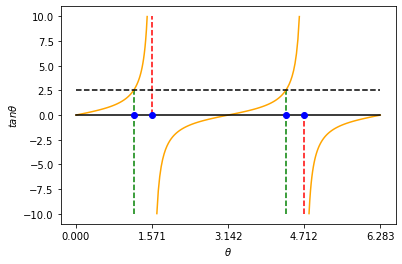
\includegraphics[width=\columnwidth]{tanx.png}
    \caption{$tan\theta$ with $m=2.5$}
    \label{fig:my_label}
\end{figure}

This gives two cases,
\begin{enumerate}
    \item when $\theta\in \left[0,\dfrac{\pi}{2}\right]\cup\left[\dfrac{3\pi}{2},2\pi\right]$
    \begin{align}
        \tan\theta&\geq m\\
        \implies \theta &\in [\tan^{-1}m, \pi/2]
    \end{align}
    \item when $\theta \in \left[\dfrac{\pi}{2}, \dfrac{3\pi}{2}\right]$
    \begin{align}
        \tan\theta&\leq m\\
        \implies \theta &\in [\pi/2, \pi+\tan^{-1}m]
    \end{align}
\end{enumerate}
\begin{align}
    \therefore \theta &\in [\tan^{-1} m, \pi+\tan^{-1} m]
\end{align}

$\theta$ will have a uniform probability distribution function: 
\begin{align}
    f(\theta)=\nonumber
    \begin{cases}
    0 &\text{if } \theta<0\\
    \dfrac{1}{2\pi} & \text{if } 0\leq\theta\leq2\pi\\
    0 &\text{if } \theta>2\pi
    \end{cases}
\end{align}
The shaded region of the figure below represents the required probability. 
\begin{align}
    \pr{\arctan m\leq\theta\leq\tan^{-1} m +\pi}\nonumber\\
    =\displaystyle\int\limits_{\tan^{-1} m}^{\pi + \tan^{-1} m} f(\theta) \,d\theta
\end{align}
\begin{align}
    &=\displaystyle\int\limits_{\tan^{-1} m}^{\pi + \tan^{-1} m} \frac{1}{2\pi} \,d\theta\\
    &=\frac{\pi}{2\pi}\\
    &=\frac{1}{2}
\end{align}
\begin{figure}[h!]
    \centering
    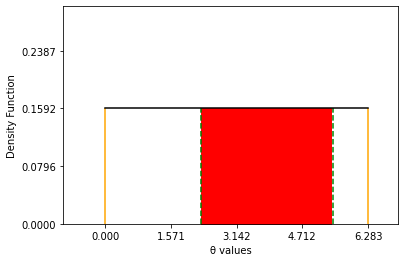
\includegraphics[width=\columnwidth]{distribution_2.png}
    \caption{Distribution function of $\theta$}
    \label{fig:my_label}
\end{figure}\\
\\ $\therefore$ option (c) is correct.
\end{document}

